\documentclass[a4paper,14pt]{article}
\usepackage{amsmath}
\usepackage[utf8]{inputenc} % 
\usepackage{graphicx}
\graphicspath{{img/}}
\DeclareGraphicsExtensions{.png,.jpg}
\usepackage{multicol}

\usepackage[russian]{babel} % правила переноса
\usepackage[left=2cm,right=2cm,
top=2cm,bottom=2cm,bindingoffset=0cm]{geometry} % для изменения размеров полей документа
\usepackage{commath}
\usepackage{listings}
\usepackage[framed,numbered,autolinebreaks,useliterate]{mcode}

\begin{document}

%%%%%%%%%%%%%%%%%%%%%% Титульный лист %%%%%%%%%%%%%%%%%%%%%%

\begin{titlepage}
	\newpage
	
	\begin{center}
		Санкт-Петербургский государственный политехнический 
		университет Петра Великого \\
		\vspace{1cm}
		Кафедра компьютерных систем и программных технологий\\*
%		\hrulefill
	\end{center}
	
	\vspace{8em}
	
	\begin{center}
		 Отчёт по лабораторной работе №5
	\end{center}
	
	\vspace{2.5em}

	\vspace{6em}
	\flushleft{Выполнила студентка гр.33501/3: Ивашкевич О.А.}

	\flushleft{Преподаватель: Богач Н.В.}
	\vspace{\fill}
	
	\begin{center}
		Санкт-Петербург
		
		 2017
	\end{center}
	
\end{titlepage}

\tableofcontents

\newpage

\part*{Лабораторная работа №5. Частотная и фазовая модуляция}
\setcounter {section}{0}
\setcounter {equation}{0}
\setcounter {figure}{0}
\section{Цель работы}
\hspace{0,5cm}   Изучение частотной и фазовой модуляции/демодуляции сигнала.
\section{Постановка задачи}
\begin{enumerate}
\item Сгенерировать однотональный сигнал низкой частоты.
\item  Выполнить фазовую модуляцию/демодуляцию сигнала, используя встроенную функцию MatLab pmmod, pmdemod.
\item Получить спектр модулированного сигнала.
\item Выполнить частотную модуляцию/демодуляцию, используя встроенные функции MatLab fmmod, fmdemod.
\end{enumerate}

\section{Теоретическое обоснование}

\subsection{Угловая модуляция}
Частотная и фазовая модуляция тесно связаны друг с другом, благодаря чему и получили общее название <угловая модуляция> (УМ; английский термин - angle modulation).\\

\subsection{Фазовая модуляция}
Пусть модулирующий сигнал определяет начальную фазу несущего колебания:

\[
	\phi(t) = kS_M(t).
\]

Тогда мы получаем сигнал с \textit{фазовой модуляцией} (ФМ; английский термин — phase modulation, PM):

\[
	S_{PM} (t)=A cos(\omega_0t + kS_M(t)).
\]
Весь аргумент функции $cos$, взятый целиком, называется \textit{полной фазой} колебания:\\

$\Psi (t)=\omega _{0}(t)+ks_{M}(t)$.\\

Круговая частота колебания по определению представляет собой скорость изменения начальной фазы. Для колебания с угловой модуляцией вводится понятие мгновенной частоты, равной производной от полной фазы по времени:\\

$\omega (t)=\frac{d\Omega}{dt}=\omega _{0}+k\frac{ds_{M}}{dt}$.\\

Итак, в случае фазовой модуляции изменяется не только начальная фаза, но и мгновенная частота колебания.\\

Соответственно, полная фаза может быть найдена путем интегрирования мгновенной частоты:\\

$\Psi (t)=\int \omega \left({t}^{\prime }\right)d{t}^{\prime }$.\\

\subsection{Частотная модуляция}

Введем понятие частотной модуляции, при которой модулирующий сигнал линейно связан с мгновенной частотой колебания:

\[
	\omega(t) = \omega_0 + kS_M(t).
\]

Добавка в виде константы $\omega _{0}$ необходима для того, чтобы сделать колебание высокочастотным.\\

Полная фаза находится путем интегрирования:\\

$\Psi (t)=\omega _{0}(t)+k\int s_{M}({t}^{\prime })d{t}^{\prime }+\phi _{0}$.\\

Здесь $\phi _{0}$ - произвольная постоянная интегрирования.\\

Наконец, сам ЧМ-сигнал имеет следующий вид:\\

$s_{ЧМ}(t)=Acos(\omega _{0}(t)+k\int s_{M}({t}^{\prime })d{t}^{\prime }+\phi _{0})$.\\

Как видим, начальная фаза колебаний при частотной модуляции претерпевает изменения, пропорциональный интегралу от модулирующего сигнала:\\

$\phi (t)=k\int s_{M}({t}^{\prime })d{t}^{\prime }+\phi _{0}$.\\

Таким образом, частотная и фазовая модуляции оказываются взаимосвязанными: если изменяется начальная фаза колебания, изменяется и его мгновенная частота, и наоборот. По этой причине два этих вида модуляции и объединяют под обзим названием <<угловая модуляция>>.\\

\section{Ход работы}
\subsection{Фазовая модуляция/демодуляция}
Для создания угловой модуляции используются функции  pmmod (фазовая модуляция) и fmmod (частотная модуляция).
Генерация гармонического сигнала и его фазовая модуляция:

\begin{lstlisting}
Ds =   4000; 
Fc = 100;
t = 0 : 1/Fs: 0.1; 
A = 2; 
F = 30;
s = A * sin(2*F*pi*t);
x 	= pmmod(s,Fc,Fs,1);
xd 	= pmdemod(x,Fc,Fs,1);
\end{lstlisting}

\newpage
Ниже приведен полученный модулированный сигнал во временной и частотной областях.


\begin{figure}[h]
\begin{multicols}{1}
\hfill
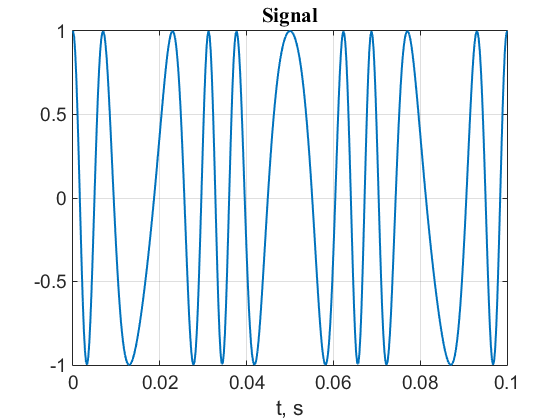
\includegraphics[width=90mm]{ph}
\hfill
\caption{Модулированный сигнал}
\label{figBottom}
\hfill
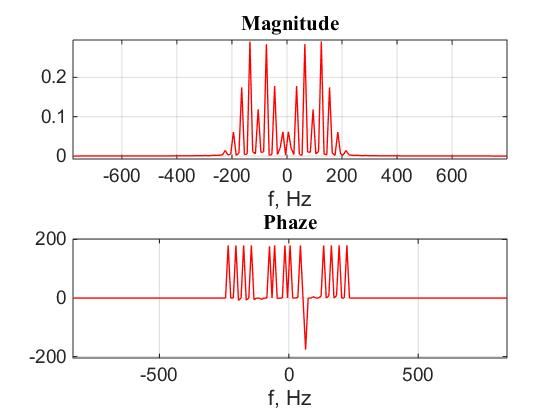
\includegraphics[width=100mm]{ph_spec}
\hfill
\caption{Спектры модулированного сигнала}
\label{figDown}
\end{multicols}
\end{figure}


Результат демодуляции сигнала:

\begin{figure}[h]
\begin{multicols}{1}
\hfill
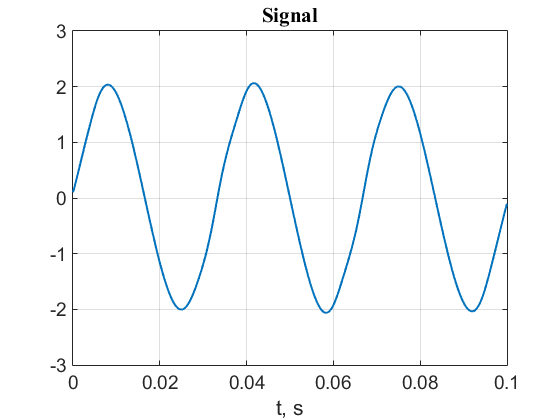
\includegraphics[width=90mm]{phd}
\hfill
\caption{Демодулированный сигнал}
\label{figBottom}
\hfill
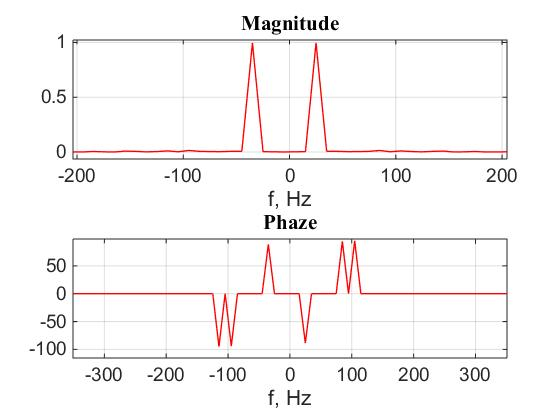
\includegraphics[width=100mm]{phd_spec}
\hfill
\caption{Спектры демодулированного сигнала}
\label{figDown}
\end{multicols}
\end{figure}

\newpage
\subsection{Частотная модуляция}

\begin{lstlisting}
y 	= fmmod(s,Fc,Fs,15);
dy 	= fmdemod(y,Fc,Fs,15);
\end{lstlisting}

Ниже приведен полученный модулированный сигнал во временной и частотной областях.

\begin{figure}[h]
\begin{multicols}{1}
\hfill
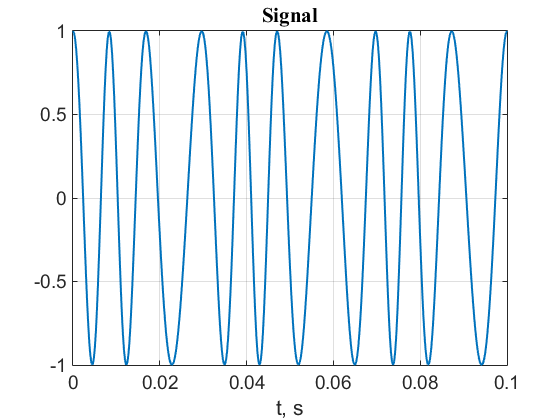
\includegraphics[width=90mm]{fr}
\hfill
\caption{Модулированный сигнал}
\label{figBottom}
\hfill
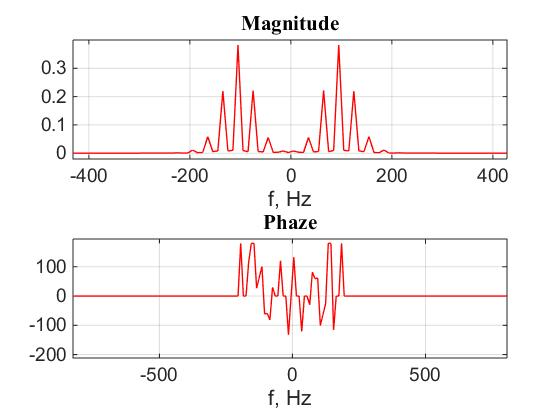
\includegraphics[width=90mm]{fr_spec}
\hfill
\caption{Спектры модулированного сигнала}
\label{figDown}
\end{multicols}
\end{figure}

Результат демодуляции сигнала:

\begin{figure}[h]
\begin{multicols}{1}
\hfill
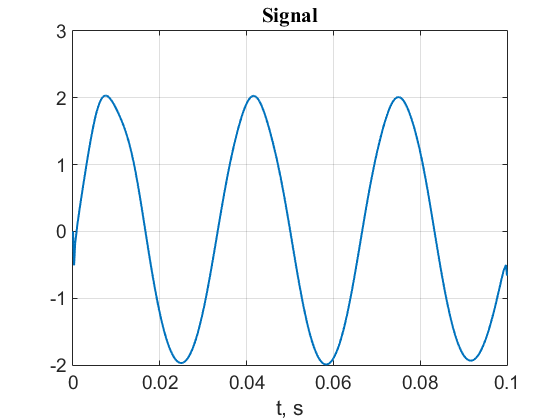
\includegraphics[width=90mm]{frd}
\hfill
\caption{Демодулированный сигнал}
\label{figBottom}
\hfill
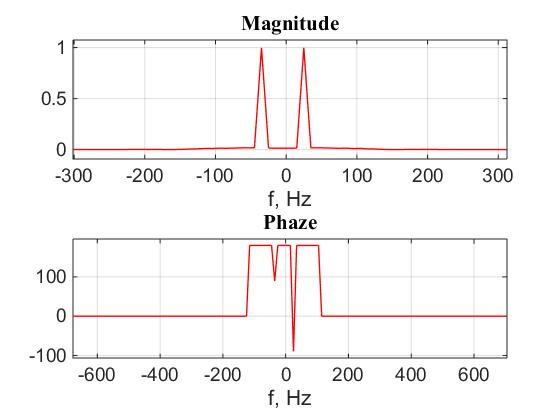
\includegraphics[width=100mm]{frd_spec}
\hfill
\caption{Спектры демодулированного сигнала}
\label{figDown}
\end{multicols}
\end{figure}


\section{Выводы}
\hspace{0,5cm} 
По итогам данной работы было получено, что из-за увеличению ширины спектра сигнала угловая модуляция обладает большей помехоустойчивостью по сравнению с амплитудной.К сожалению, большая ширина спектра является недостатком данной модуляции. В современном мире, использование данного типа модуляции находится  в системах телевизионного вещания, системах спутникового теле- и радиовещания и в сотовой телефонной связи.
\end{document}